\documentclass{article}
\usepackage{geometry}
\geometry{a4paper}
\usepackage{ctex}%中文
\usepackage{graphicx}%图片
\usepackage{multirow}%表格
\usepackage{amsmath}%公式,公式换行等时候会用到
\usepackage{amsmath}
\usepackage{amsfonts}%特殊符号,比如说实数集
\usepackage{subfigure} 
\title{最优化学习笔记3最优建模}
\author{BD S}
\begin{document}
\maketitle
\tableofcontents
\newpage
一般来说,建模的过程通常分为:定义目标,查找相关文献、建立模型收集数据、初始测试以及验证模型。
\section{建模技术}
\subsection{目标函数的设计}
\subsubsection{最小二乘以及正则化}
1.最小二乘法。
形式一般是
$$
\min\limits_{x \in \mathbb{R}^n} \sum\limits_{i=1}^m (b_i-\phi_i(x))^2
$$
$l_2$范数是光滑可微的,会给目标函数带来较好的性质,同时$l_2$范数对于某种误差的处理有最优性。当然也不一定是二范数,一范数、无穷范数都是可以的

2.正则化。
在建模的时候,我们往往需要借助于想要得到的解的性质。比如想要得到一个稀疏的解,就是
$$
\min\limits_{x \in \mathbb{R}^n} \sum\limits_{i=1}^m (b_i-\phi_i(x))^2+\mu||x||_0
$$
甚至在图像处理中,希望其某个变换域是稀疏的,那么就有
$$
\min\limits_{x \in \mathbb{R}^n} \sum\limits_{i=1}^m (b_i-\phi_i(x))^2+\mu||W(x)||_0
$$
一般这个W可以是全变差、小波变换等。
后面这些多出来的项就可以叫做正则项,也可以理解为惩罚项。
\subsubsection{极大似然估计}
关于极大似然估计的补充。对于一个函数$p(x;\theta)$,$x$是事件$\theta$是概率。如果已知概率,事件是变量(等待我们去做),那就是一个概率函数。如果已知事件,未知概率,那就是一个似然函数。
举个例子,从一个箱子里抽球,已知抽到黑球的概率是70\%,那么就可以得到概率函数$p(black)=0.7$。如果未知概率,但是已经从箱子里面独立的抽了100次球,其中70次是黑球,那么就可以得到似然函数$p^{70}(1-p)^{30}$,当这个似然函数最大的时候,就是我们估计出的概率,很显然求导得到是0.7。

很多数据来自未知的概率分布,从数据反推分布的具体形式是非常重要的课题。通过最大化似然函数,使得观测数据尽可能服从假定的模型。
可以根据实际结果列出似然函数
$$
L(x)=\prod_{i=1}^n p(a_i;x)
$$
$x$某种意义上就是概率,某一事件对应的概率。要最大化这个函数$lnL(x)$
考虑一个最大化问题
$$\max\limits_{x \in \mathbb{X}} l(x)=lnL(x)$$
假设数据是服从高斯分布的,就是$a_i\sim N(\mu,\sum)$,其中均值$\mu$和协方差矩阵$\sum$都是未知的。
就有$$
p(a;x)=\frac{1}{\sqrt{(2\pi)^p det(\sum)}}\exp[-\frac{1}{2}(a-\mu)^T(\sum)^{-1}(a-\mu)]
$$
概率依次相乘构造出优化问题。
\subsubsection{松弛}
比如说吧$l_0$范数松弛为加权$l_1$范数,或者说用一个结构简单的下界来代替原来的函数,拉格朗日函数某种程度上也是松弛。
\subsection{约束的设计}
问题本身的物理性质。
也可以等价转换。把约束变成目标,把目标部分化为约束。
还可以做松弛。比如说用盒约束$x \in [0,1]$代替整数约束$x \in \{0,1\}$

\section{回归分析}
经典的监督学习主要分为回归和分类两类问题。
一般的回归模型可以写成$$b=f(a)+\epsilon$$
$a \in \mathbb{R}^d$为自变量,$b \in \mathbb{R}$为应变量,$\epsilon \in \mathbb{R}$为模型的噪声或者误差。实际过程中,我们只能观测到$a$和$b$的值,而误差未知,函数$f$的具体形式也未知了。回归模型的任务是利用$m$个观测值$(a_i,b_i)$来求解出$f$的具体形式。

但是如果简单的使用插值的方式来构造出一个很复杂很丑$f$,虽然训练集拟合的很好,但是测试集的效果会很差,这就是过拟合了。但是如果$f$的形式过于简单,就无法表述$a$和$b$的关系,这就是欠拟合。

为了缩小$f$的范围进行参数化,模型变为$b=f(a;x)+\epsilon$,缩小了$f$的范围,但是我至今还是不太懂。
\subsection{线性回归模型}
线性回归模型可以说是最简单的了。设$(w_i,b_i)$分别为观测到的自变量和响应变量,且不同数据点相互独立。则对每个数据点
$$
b_i=w_{i1}x_1+w_{i2}x_2+\dots+w_{i,n-1}x_n+x_n+\epsilon_i
$$
其中$x_i$是待确定的参数。(注意为了计算方便,最后一项没有权重)
那么如果令$a_i^T=(w_1,w,2,\dots,w_n-1,1),x=(x_1,x_2,\dots,x_{n-1},x_n)……T$
那么上述的回归模型可以简写为$$b_i=a_i^Tx+\epsilon_i$$
再进一步,输入的训练集可以写成一个$m*n$的矩阵A,将标签$b_i$和噪声$\epsilon_i$写成向量形式$b$和$\epsilon$,即
$$
b=Ax+\epsilon
$$
假设$\epsilon$是服从高斯分布的,那么这个模型的概率密度函数就是
$$
p(b_i|a_i;x)=\frac{1}{\sqrt{2\pi \sigma^2}}exp(-\frac{(b_i-a_i^Tx)^2}{2\sigma^2})
$$
那么对数似然函数就是
$$
l(x)=ln\prod_{i=1}^m p(b_i;a_i;x)=-\frac{m}{2}ln(2\pi)-m ln\sigma-\sum_{i=1}^m \frac{(b_i-a_i^Tx)^2}{2\sigma^2}
$$
其中关于$\sigma$,我们并不关心它的具体大小,去掉常数项就得到了一个最小二乘问题
$$
\min\limits_{x \in \mathbb{R}^n} \frac{1}{2} ||Ax-b||^2_2
$$

此外,当$\sigma$不是高斯白噪声的时候,求解线性回归模型和高斯白噪声问题并不等价。有时候根据噪声构造出来的问题是最小一乘问题。
$$
\min\limits_{x\in \mathbb{R}^n} ||Ax-b||_1
$$
\subsection{正则化线性回归模型}
当数据集的特征数量大于样本总量的时候,问题的解不唯一,需要正则项来选出性质不同的解。
\subsubsection{Tikhonov正则化}
为了平衡模型的拟合性质和解的光滑性,添加$l_2$范数平方为正则项。
实际上就是在求解一个这样的问题
$$
\min\limits_{x \in \mathbb{R}^n} \frac{1}{2} ||Ax-b||^2_2+\mu ||x||^2_2
$$
由于加入了正则项,所以这个目标函数会是个强凸函数,解的性质会得到改善。
同理也可以加约束
$$
\min\limits_{x \in \mathbb{R}^n} \ \frac{1}{2} ||Ax-b||^2_2
$$
$$
s.t. \ ||x||_2 \le \sigma
$$
\subsubsection{LASSO问题及其变形}
可以是这样
$$
\min\limits_{x \in \mathbb{R}^n} \frac{1}{2} ||Ax-b||^2_2+\mu ||x||_1
$$
是这样
$$
\min\limits_{x \in \mathbb{R}^n} \ \frac{1}{2} ||Ax-b||^2_2
$$
$$
s.t. \ ||x||_1 \le \sigma
$$
还可以这样
$$
\min\limits_{x \in \mathbb{R}^n} \ ||x||_1 
$$
$$
s.t. \ ||Ax-b||_2 \le v
$$
传统的LASS0问题要求x是一个稀疏解,但实际上稀疏性可能会有多个表达式。如果要求具有分组的稀疏性,那么就无法满足。可以把分量分为G个组,每个组内参数必须同时为0或非0。
那么就可以列出式子
$$
\min\limits_{x \in \mathbb{R}^n} \frac{1}{2} ||Ax-b||^2_2+\mu \sum\limits_{l=1}^G
\sqrt{n_l}||X_Il||_2
$$
其实后面那项就是由$||x||_1 $转换过来的,因为$l_1$范数是绝对值的和,分成G个组绝对值的和,每个部分也是一个$l_1$范数,也就是$\sum\limits_{l=1}^G$。
甚至还有不当人的
$$
\min\limits_{x \in \mathbb{R}^n} \frac{1}{2} ||Ax-b||^2_2+\mu_1\sum\limits_{l=1}^G
\sqrt{n_l}||X_Il||_2+\mu_2 ||x||_1
$$
简直稀疏到家了。
甚至还可以要求在某种变换下的稀疏性,比如
$$
\min\limits_{x \in \mathbb{R}^n} \frac{1}{2} ||Ax-b||^2_2+\mu_1\sum\limits_{l=1}^G
\sqrt{n_l}||X_Il||_2+\mu_2 ||Fx||_1
$$
$$
\min\limits_{x \in \mathbb{R}^n} \frac{1}{2} ||Ax-b||^2_2+\mu_1\sum\limits_{l=1}^G
\sqrt{n_l}||X_Il||_2+\mu_2 ||x_i-x_{i-1}||_1
$$
\section{逻辑回归}
刚刚讲的是回归,现在讲分类,也就是逻辑回归。逻辑回归简单、可并行化、可解释强深受工业界喜爱。给定一个特征值$a$,逻辑回归假设这个样本属于类别1的概率
$$
p(1|a;x)=P(t=1|a;x)=\theta(a^Tx)
$$
\subsection{logistic分布}
分布函数和密度函数分别为
$$F(x)=P(X \le x)=\frac{1}{1+e^{-(x-\mu)/ \gamma}}$$
$$f(x)=F(X \le x)=\frac{e^{-(x-\mu)/ \gamma}}{\gamma (1+e^{-(x-\mu)/ \gamma})^2}$$
\begin{figure}[h]
    \centering
    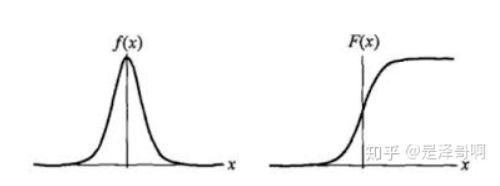
\includegraphics[width=12cm]{1.png}
    \caption{分布函数和密度函数图像}
\end{figure}
\subsection{logistic回归}
比如说一个图2的二分类问题,只要符合$w_1x_1+w_2x_2+b>0$,就可以归为类别1。只要符合$w_1x_1+w_2x_2+b<0$,就可以归为类别0。
\begin{figure}[h]
    \centering
    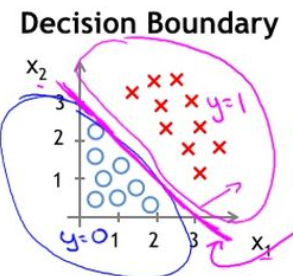
\includegraphics[width=4cm]{2.png}
    \caption{二分类问题}
\end{figure}

但是逻辑回归还要加一层,令$z=w_1x_1+w_2x_2+b$,创建一个$p(z)=0/0.5/1$,通过这个概率$p(z)$的大小来判断类别。引入对数几率函数,
$$
y=\frac{1}{1+e^{-w^Tx+b}}
$$
其实就是上文提到的logistic分布函数
$$F(x)=P(X \le x)=\frac{1}{1+e^{-w^Tx+b}}$$
这样的作用是,对于大于0的$z$,取概率大于$p(z)>0.5$分为第一类$y=1$,反之取小于,分为第二类$y=-1$。
取到$y=1$和$y=-1$的概率之和为1,而如果加上一项$y$,变成
$$F(x)=P(X \le x)=\frac{1}{1+e^{-y(w^Tx+b)}}$$
这个就很恐怖了,两种情况都能用这个式子来描述,那写优化问题也很方便了。

优化问题就是
$$\min\limits_{x \in \mathbb{R}^n}\sum\limits_{i=1}^m ln(1+e^{-y(w^Tx+b)})$$
还可以加上1范数或2范数的正则项。
假设数据集里面的$\{a_i,b_i\}$是由随机变量对$\{\alpha,\beta\}$产生,那么损失函数就可以学成均值形式
$$E[{x \in \mathbb{R}^n}\sum\limits_{i=1}^m ln(1+e^{-y(w^Tx+b)})]$$
加上正则项也可以抽象为更一般的优化问题或者它的离散版本
$$\min\limits_{x \in \mathbb{R}^n} f(x)+\lambda r(x)$$

\section{支持向量机SVM}
这也是一种二分类模型,给定一个训练集$D$中的样本点$(a_i,b_i)$,且$a_i \in \mathbb{R}^n,b \in \{-1,1\}$,那么可以通过一个超平面来划分,当然这样的超平面会有很多个。
比较理想的超平面肯定是要离数据点远一点的,这样才会有较好的鲁棒性。

点$\omega_0$到平面$\omega^Tx+y=0$距离的公式为$$
d=\frac{x^T\omega_0+y}{||x||^2}
$$
对于一系列的训练集$(a_i,b_i)$,如果分类正确,就有$b_i(a_i^Tx+y)>0$
而我们也可以得到优化问题
$$
\max\limits_{x,y,\gamma} \gamma
$$
$$
s.t. \ \frac{b_i(a_i^Tx+y)}{||x||_2} \ge \gamma 
$$
对于$x,y$以相同倍数缩小是可以接收的,那么不妨设$||x||_2=\frac{1}{\gamma}$,得到了
$$
\min\limits_{x,y}  ||x||_2
$$
$$
s.t. \ b_i(a_i^Tx+y) \ge 1
$$
在此基础上,引入误分点的概念。就引入一个$\zeta_i$使得约束变为,
$$
s.t. \ b_i(a_i^Tx+y) \ge 1-\zeta_i
$$
因为有一部分点还是得被分类错,这里的$\zeta_i$越大,就代表被误分的越离谱
所以新的目标函数就是
$$
\min\limits_{x,y} \  ||x||_2^2+\mu \sum\limits_{i=1}^m \zeta_i
$$
要让误分量越小越好。
$$
\min\limits_{x,y} \  ||x||_2^2+\mu \sum\limits_{i=1}^m \zeta_i
$$
$$
s.t. \ b_i(a_i^Tx+y) \ge 1-\zeta_i, \ \zeta_i \ge 0
$$
这个优化问题也等价于无约束优化问题
$$
\min\limits_{x,y} \ \frac{1}{2}||x||_2^2+\mu \sum\limits_{i=1}^m \max\{ 1-b_i(a_i^Tx+y),0\}
$$
但是这个就不能求微分了,也有人把二范数换成1范数,为了去掉冗余特征。

\section{概率图模型}
概率图模型是概率论里面的一个重要的概念,它是一种利用图结构来描述多元随机变量之间条件独立关系的概率模型。图的每个节点(node)都关联了一个随机变量,而图的边(edge)则被用于编码这些随机变量之间的关系。根据图是有向的还是无向的,我们可以将图的模式分为两大类——贝叶斯网络( Bayesian network)和马尔可夫网络(Markov networks)。
\subsection{贝叶斯网络}
贝叶斯网络的一个典型案例是所谓的「学生网络(student network)」,它看起来像是这样:
\begin{figure}[h]
    \centering
    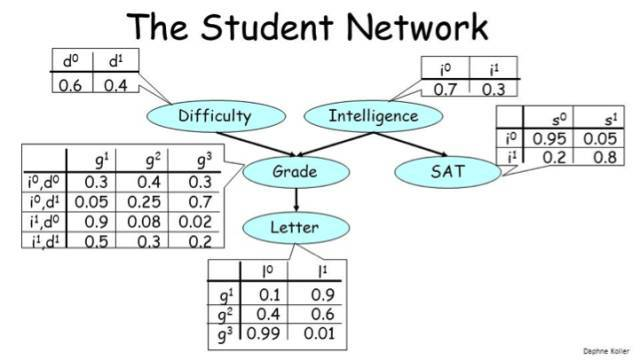
\includegraphics[width=10cm]{1.jpeg}
\end{figure}

这个图描述了某个学生注册某个大学课程的设定。该图中有 5 个随机变量:

1.课程的难度(Difficulty):可取两个值,0 表示低难度,1 表示高难度;

2.学生的智力水平(Intelligence):可取两个值,0 表示不聪明,1 表示聪明;

3.学生的评级(Grade):可取三个值,1 表示差,2 表示中,3 表示优;

4.学生的 SAT 成绩(SAT):可取两个值,0 表示低分,1 表示高分;

5.在完成该课程后学生从教授那里所得到的推荐信的质量(Letter):可取两个值,0 表示推荐信不好,1 表示推荐信很好。

该图中的边编码了这些变量之间的依赖关系:
学生的 Grade 取决于课程的 Difficulty 和学生的 Intelligence;
而 Grade 又反过来决定了学生能否从教授那里得到一份好的 Letter;
另外,学生的 Intelligence 除了会影响他们的 Grade,还会影响他们的 SAT 分数。
注意其中箭头的方向表示了因果关系——Intelligence 会影响 SAT 分数,但 SAT 不会影响 Intelligence。

最后,让我们看看与每个节点关联的表格,它们的正式名称是条件概率分布(CPD/conditional probability distribution)。注意两点,贝叶斯网络的一个基本要求是图必须是有向无环图(DAG/directed acyclic graph),且每一行的概率和为1。

\subsection{马尔可夫网络}
正如贝叶斯网络有CPD一样,马尔可夫网络也有用来整合节点之间的关系的表格。但是,这些表格和 CPD 间有两个关键差异。

首先,这些值不需要总和为1,也就是说这个表格并没有定义一个概率分布。它只是告诉我们值更高的配置有更高的可能性。其次,其中没有条件关系。它与所涉及到的所有变量的联合分布成正比,这与 CPD 中的条件分布不同。

这样得到的表格被称为“因子(factor)”或“势函数(potential function)”,使用希腊字母φ 表示。比如,我们可以使用下面的势函数来描述变量 A、B 和 C 之间的关系,其中 C 是 A 和 B 的“软”异或(XOR),也就是说:如果 A 和 B 不一样,那么 C 很可能为 1;如果 A 和 B 一样,那么 C 很可能为 0。
\begin{figure}[h]
    \centering
    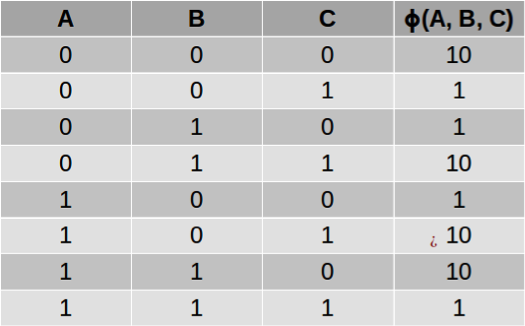
\includegraphics[width=5cm]{3.png}
\end{figure}

\subsection{问题设置}
比如说有向图,给定了一系列的已知条件比如说SAT分数,各个课程的成绩,以及推荐信。从而来估计每一个连接之间的概率。
\subsection{条件独立}
在贝叶斯网络的图中,可以看到难度与智力是独立的,SAT和GRADE也是独立的,它们之间没有互相连接。
\subsection{接下来回到课本}
一个向量$X=(X_1,X_2,\dots,X_n)$,假设其中的每一个量都有m种取值的可能。那么首先可以得出
$$
P(X=x)
=P(X_1=x_1)P(X_2=x_2|X_1=x_1)\dots
$$
第一步是$P(X_1=x_1)$的概率,第二步时在$P(X_1=x_1)$条件下$P(X_2=x_2)$的概率,
依次相乘下去,会得到
$$
P(X=x)=\prod\limits_{k=1}^n P(X_k=x_k|X_1=x_1,X_2=x_2,\dots,X_n=x_n)
$$
已知有n个变量,每一个量都有m种取值的可能,那么就需要$(m^n-1)$个参数才能确定相应的概率分布。当然,如果变量之间存在独立性,那么需要的参数就少很多了。
不妨做以下假设,对于三个二值变量$x_1,x_2,x_3$。假设,在$x_2$已知确定的时候,$x_1$和$x_3$互相独立。
那么就可以有
$$
P(x_1=x_1|x_2=x_2,x_3=x_3)=P(x_1=x_1|x_2=x_2)
$$
$$
P(x_3=x_3|x_2=x_2,x_1=x_1)=P(x_3=x_3|x_2=x_2)
$$
进一步可以得到
$$
P(X=x)=P(x_1=x_1)P(x_1=x_1|x_2=x_2)P(x_3=x_3|x_2=x_2)
$$
这就是$1+2^1+2^=5$个参数就可以确定联合分布。

协方差矩阵,计算的是两个随机变量间的关系,那么如果有n个随机变量呢,两两计算cov需要计算次,因此用矩阵来表示这个计算就得到协方差矩阵了。我们的目标就是计算真实的协方差矩阵

这部分讲的不清楚,不想写下去了。
\section{相位恢复}
这个有点像压缩感知。主要可以用来恢复信号,甚至相位信息比模长信息更重要。
给定一个复信号$x=(x_0,x_1,x_2,\dots,x_{n-1})^T \in \mathbb{C}^n$
以及采样数$m$,我们可以逐分量定义线性变换。
$$(A(x))_k=a_k^T x, k=1,2,\dots,m$$
注意,这个复信号x才是我们要去求的。

举个例子,对于这个$a_k$,如果变换$A$是傅里叶变换的话,那么
$$a_k=(e^{2 \pi i \frac{k-1}{n}t})^{n-1}_{t=0}$$

那么接下来就是真正写优化问题了,观测到的振幅为$b_k$的话,那么就有
$$
b_k^2=|a_k^T x|^2,\ k=1,2,\dots,m.
$$

这是个二次方程组,求解起来是NP难的,所以转换模型。
\subsection{最小二乘模型}
$$
\min\limits_{x \in \mathbb{C}^n} \sum\limits^m_{i=1}(b_k^2-|a_k^T x|^2)^2
$$
也可以构造以下非光滑模型
$$
\min\limits_{x \in \mathbb{C}^n} \sum\limits^m_{i=1}(b_k^2-|a_k^T x|^2)^2
$$
\subsection{相位提升}
难以求解主要是有二次项,不妨这样做
$|a_k^T x|^2=Tr(xx^Ta_ia_i^T)$
令$X=xx^T$,这个X的秩为1,两个向量外积的秩最多为1。
所以可以写出优化问题
$$
\min\limits_{X} \ \ \ \ \ \ \  \ rank(X),
$$
$$
s.t. \ \ Tr(Xa_ia_i^T)=b_i^2,i=1,2,\dots,m,
$$
$$
X \succeq 0
$$
把向量变为矩阵变量,这在某种程度上是一个提升。
但是秩的计算比较复杂,采用核函数进行松弛,得到了
$$
\min\limits_{X} \ \ \ \ \ \ \  \ Tr(X),
$$
$$
s.t. \ \ Tr(Xa_ia_i^T)=b_i^2,i=1,2,\dots,m,
$$
$$
X \succeq 0
$$
\section{主成分分析}
高维点在低维子空间中表达的方法。给定n个样本,定义$A=[a_1,a_2,\dots.a_n]$
不失一般性,假设A的行为和为0。(相当于逐元素减去该行的平均值)

将高维的点投影到低维中去,数据点$a_i$在$X$张成的子空间投影为$P_X(x_i)=XX^Ta_i$
需要找到一个最优的$X$使得投影后的方差最大。协方差矩阵的值为$\frac{1}{n} \sum\limits_{i=1}^n X X^T a_i (XX^Ta_i)^T=\frac{1}{n}  X X^T A (XX^TA)^T$

得到优化问题,$$max \ Tr(X^T AA^TX) \ \  \ s.t. X^TX=I$$
不难发现,这个问题就是求$AA^T$
从大到小排列的d个特征值对应的特征向量。

对于某一点的重构误差就是$||XX^Ta_i-a_i||$,那么从重构误差的角度来看的话,
$$
\sum\limits_{i=1}^n ||XX^Ta_i-a_i||^2_2=||XX^TA-A||^2_F=-Tr(X^TAA^TX)+Tr(A^TA)
$$
使得重构误差平方最小就是求解优化问题
$$max \ -Tr(X^TAA^TX)+Tr(A^TA) \ \  \ s.t. X^TX=I$$

\section{矩阵分离问题}


\end{document}